% \section{Energetic particles in the heliosphere}
% \label{sec:particles_heliosphere}

% \begin{figure}
% 	\centering
% 	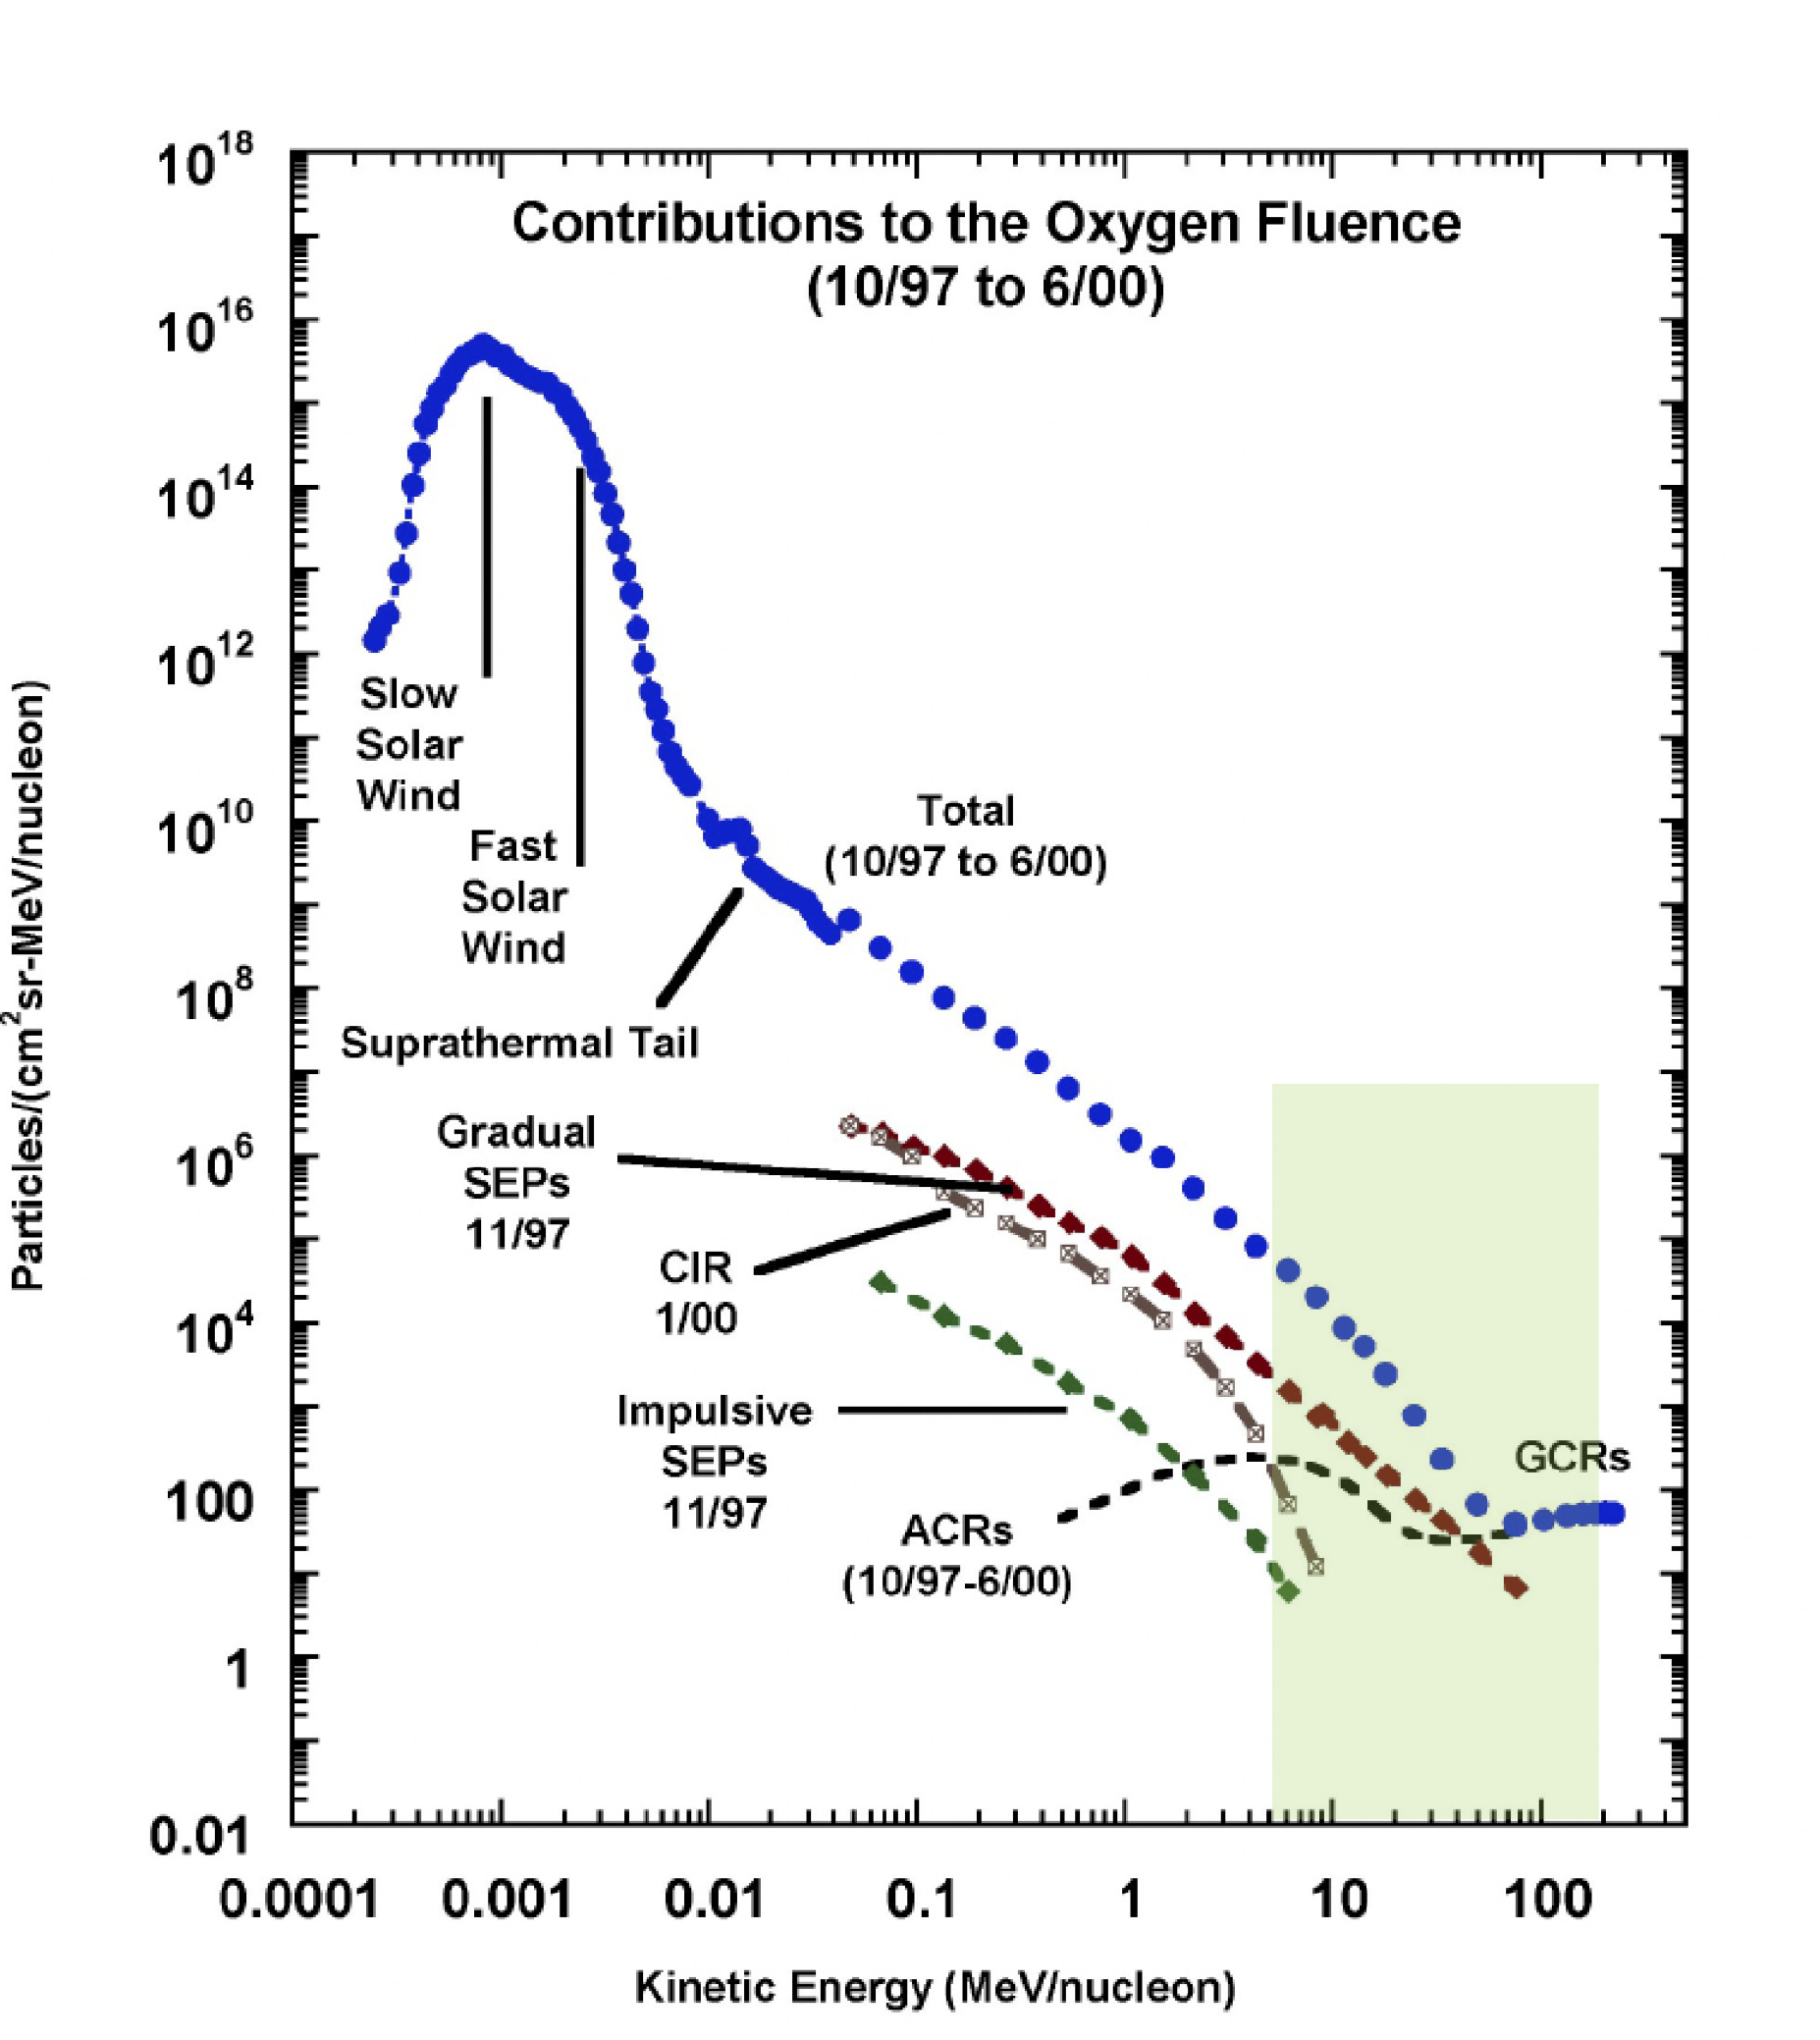
\includegraphics[width = 0.8\textwidth]{images/heliospheric_particle_spectra_color.png}
% 	\caption[Energy spectra of oxygen ions in near-Earth space]{The typical oxygen spectra in the interplanetary space near Earth, indicating the contributions of different particle populations, particularly in the energy range between few MeV/nuc and few hundreds MeV/nuc (shadow region), where \acs{SEP}, \acs{ACR} and \acs{GCR} coexist. The spectra of other particles species such as, helium and proton have the similar shape but a different flux level in corresponding energy region. The figure is adapted from \citep{Mewaldt-2001}}
% 	\label{Fig:Oxygen_spectra_heliosphere}
% \end{figure}

% Heliosphere is a vast, bubble-like region in the space that envelops the Sun. This region is moving in the \ac{ISM} with a speed of about 25 km/s \citep{McComas2015ApJS}. Such a cavity is created by the sun and governd by its magnetic field and solar wind; a substantial amount of plasmas of various particle populations fill this space. The particle populations could be identified from Fig.\ref{Fig:Oxygen_spectra_heliosphere} which is adapted from \citet{Mewaldt-2001}. Based on the accumulated measurement of oxygen by \ac{ACE} between 1997 and 2000, the fluence oxygen spectrum which spans over more than 7 orders of magnitude from keV/nuc to GeV/nuc provides clear insight into the lower energy particles including slow solar wind, fast solar wind, suprathermal tail, and high energy particles composed of \ac{SEP}, \ac{ACR}, and the extremely high energy \ac{GCR}. 
% Among them \acs{GCR} originate from distant sources outside the solar system, while \acs{ACR} sources located near the boundary of heliosphere. The remaining energetic particles are the parrticle accelerated and generated inside of the heliosphere at the multiple locations, including solar surface, interplanetary space and even the planet for instance Jupiter.

% Solar wind is a stream of charged particles released from the solar corona, the upper atmosphere of the Sun. Such a group of plasam consists of mainly protons and electrons that continously flow outward and expend to about $\sim$ 100 au (differ in directions). The typical energy range of the solar wind is between 0.5 keV and 10 keV. Depending on the locations on the sun that produces the solar wind, the speed and density of solar wind might be different. For instance the fast solar wind with a typical speed between 500 and 800 kilemeters per second emits from the coronal holes which are funnel-like regions of open field lines in the magnetic field and usually appear in the north and south pole of sun. Therefore, the fast solar dominate the high latitude regions. While the slow solar wind is observed to have a velocity of about 300 - 500 kilometers per second and is believed to originate from the streamer belt along the equatorial belt. The slow solar wind is more likely to be observed in the low latitude regions.

% %plasma embedding with magnetic field

% Suprathermal particles are charged ions and electrons that move about two to hundreds times faster than the solar wind particles. In the spectrum shown in Fig.\ref{Fig:Oxygen_spectra_heliosphere}, the suprathermal particles are beyond the tails of the fast solar wind and are the dominate particles between few keV to hundreds of keV. The source of suprathermal particle might be the accelerated solar wind and the remanent of the previous solar eruptions and \ac{SEP} events. Those particles play am important role in contributing seed particles for the \ac{SEP} events.

% Above the energy of suprathermal particle are the energy range that we are interested in this thesis, especially the energy range between 10 MeV/nuc and few hundred MeV/nuc where the dominated particles are \ac{SEP} (not limited to this energy range),\ac{ACR} (up to $\sim$ 100 MeV/nuc) and lower energy \ac{GCR}. The measurements we used in this study are from this energy range.

% The \ac{SEP} are the high energetic particles with energy of few keV up to $\sim$ GeV oriented from the sun and accelerated during the solar activities like solar flare and \ac{CME} driven shocks. \acs{SEP} events are recurring, short term, and intensive. Different type of \acs{SEP} events persist for different time scales from few hours to few days. Such high energy particles are one of the major threats in the space.
% %also particle from solar, accelerated by different mechanism. The enery range of \ac{SEP} are quite broad, especially depending the on where the measurement carried on. Recently \ac{SOLO} and \ac{PSP} frequently measure the hundreds keV \ac{SEP}.

% \acs{ACR} are the high energy interstellar pick-up ions \citep{Giacalone2022SSRv} which are ionized neutral interstellar atoms generated by solar UV radiation after they move cross the boundary and enter the heliosphere. Those ionizing particle are then carried by the expanding solar wind to the outer boundary of helioesphere, where they are accelerated by the termination shock and then propagate inwards. The typcial \ac{ACR} species that have been observed are proton, helium, oxygen, nitrogen, iron, neon. 

% \ac{GCR} are the fully ionized particles that is accelerated at the so-called supernova remnants \citep{Blasi2013AARv2013} which are outside of the solar system. Those high energy particles bombard Earth in a constant and slowly varying way. The complete GCR spectrum cover the energy from typical 1MeV \citep{Potgieter2013LRSP} to ZeV which is larger than the energy range in Fig.~\ref{Fig:Oxygen_spectra_heliosphere}. The \acs{GCR} is comprised of about 89\% of hydrogen, 10\% of helium, 1\% of heavier ions as well as electron, positron and antiprotons. 

% After entering the heliosphere, the transport of both cosmic rays are controled by the \ac{HMF}, hence \ac{ACR} and \ac{GCR}'s temporal variaton is highly related with the solar activities and the so-called solar modulation, which periodcally changes in 11 and 22 year periods. 


\section{Solar energetic particles}

\subsection{Two types of SEPs}


The first observation of \ac{SEP} events was made during a magnetic storm on March 1, 1942 \citep{lange1942note,forbush1942further}, during which three unusual increases in the cosmic-ray intensity were observed in ground-based ionization chambers and neutron monitors. Those increased appeared simultanously with solar flare eruptions. Later, \citet{Forbush1946} attributed such increases to the charged particles emitted from the Sun with sufficient energy to penetrate the Earth's atmosphere. Nowdays, such event are called \ac{GLE} events. The particle energies in these events exceed $\sim$ 400 MeV/nuc and pose a major threat for human health \citep{meyer1956solar,Shea2012SSRv,gopalswamy2013first,thakur2014ground, Reames2013, Mironshnichenko2013Ge}.
%Now we have known that this is the so-called \ac{GLE}, one type of the most hazard energetic particles in the space of more than 433 MeV/nuc energy, typical more than GeV. \citep{meyer1956solar,Shea2012SSRv,gopalswamy2013first,thakur2014ground, Reames2013, Mironshnichenko2013Ge}.

During first few decades after the discovery of \ac{SEP}, it was commonly believed that the generation of \acp{SEP} were highly related to the solar flare because they appeared simultanously. This is the so-called "solar flare myth" as discussed in \citep{gosling1993the}. The important role of \acp{CME} and the \ac{CME}-driven shocks that are capable of accelerating particle up to energies of few GeV have been largely underestimated,
%and its driven shocks in the generation of \ac{SEP} was largely underestimated, 
 although a considerable amount of researches focused on the characteristics of such \acp{SEP} like the duration, longitudinal distribution, the abundance of the typical elements and their association with radio burst had already indicated the existence of two types of distinct events - impulsive and gradual \ac{SEP} events \citep{kahler1978prompt,kahler1984associations,cliver1982injection,cane1986two, reames1988ApJ}.
Currently, scientists have established a classic two-class paradigm (See,Fig.~\ref{Fig:two_type_SEP} and Tab.~\ref{Tab:Two_type_SEP}) which has been widely accepted by the science community \citep{kallenrode2003current, reames2013two,Desai_Diacalone2016LRSP, Reames2021LNP}. Both acceleration mechanism and the source locations are different for the two types of \acp{SEP}.
\begin{figure}[!htb]
	\centering
	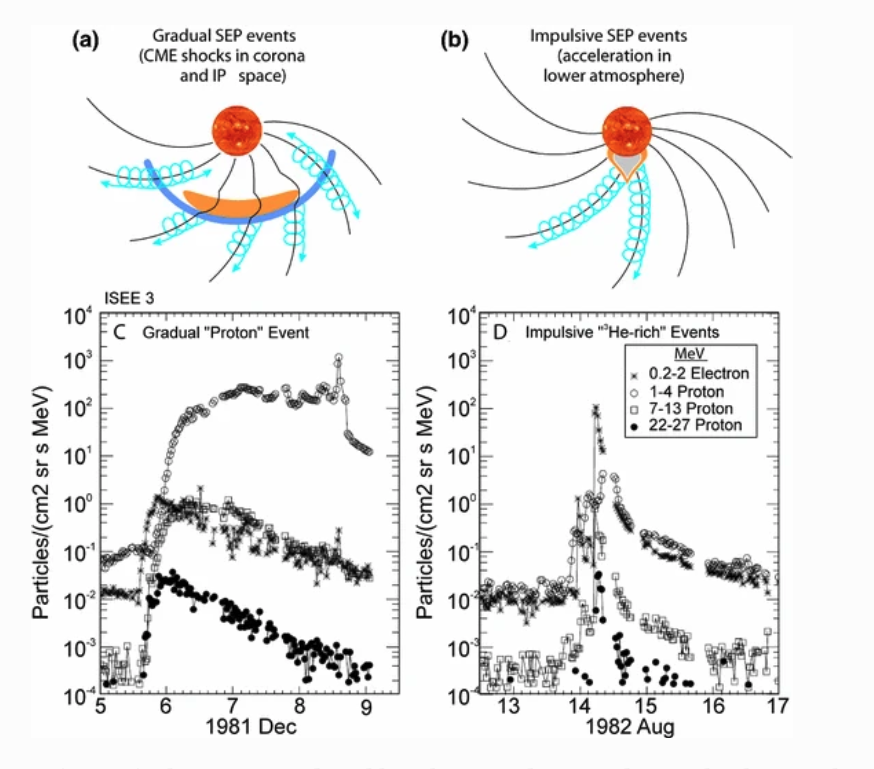
\includegraphics[width = 0.75\textwidth]{images/SEP_two_type.png}
	\caption[Two types of Solar energetic particle (SEP) event]{Two classes of \ac{SEP} events. (a) The gradual \ac{SEP} events that are associated with \ac{CME} drivens shocks in the corona or in the interplanetary space. The particles populate the \ac{IMF} lines over a wide range of longitudes. (b) The impulsive \ac{SEP} events that are associated with solar flares. Here, the particles only populate a limited range of the open \ac{IMF} lines that are well-connected to the flare site. Plots (c) and (d) are the corresonding typical proton and electron time profiles of the large gradual and small impulsive SEP events. The figure is reproduced from \citet{Desai_Diacalone2016LRSP}.}
	\label{Fig:two_type_SEP}
\end{figure}

Fig.~\ref{Fig:two_type_SEP} illustrates the established scenario of gradual (left) and impulsive (right) \acp{SEP}.
The gradual events are diffusively accelerated by the \ac{CME}-driven coronal and interplanetary (IP) shocks. Generally, a complete gradual \ac{SEP} event usually consists of a sharp increase phase as the start, a long lasting plateau and a flux peak at lower energy which indicates the arrival of the \ac{CME} at the detector. The event finishes with a decay phase and the flux returns to the quiet-time level. The whole process might persist from one day to several days. Gradual \acp{SEP} are always accompanied by type II radio bursts, which are broad and slow shift strutures in the dynamic radio spectrum which are considered as signatures of \acp{CME} and its propagtion track from the Sun to 1 au. Shocks mainly accelerate protons and heavy ions, but not electrons with the same efficiency, causing a smaller electron to proton ratio compared to impulsive \ac{SEP}. Besides, gradual \acp{SEP} events spread widely in the IP since \acp{CME} have broader longitudinal extents and can be measured by multiple detectors even if they are far away from each other. 
%In the next section, we discuss widespread events in more detail. 
The appearance frequency of gradual \acp{SEP} during the solar activiy maximum is about $\sim 100$ per year.

While a solar flare which erupts from the a solar active region is considered as the souce of an impulsive \ac{SEP} event. The strong magnetic reconnection happened during the flare eruption can accelerate particles, especially electons, up to hundred MeV. Therefore, the electrons are the dominant particles in such an event. Besides, in this senario, the particles escape from the open magnetic field and arrive at the Earth along the spiral magnetic field. i.e. the Parker spiral, \citep{Parker-1958} that is shaped by the expanding solar wind. From the Earth's point of view, the impulsive \acp{SEP} are typically located in a narrow region in the western hemisphere of the Sun. Type III radio bursts usually appear with impulsive events, rather than \acp{CME}.
The appearance frequency of impulsive \acp{SEP} during the solar activity maximum is about $\sim 10^3$ per year. The typical duration of impulsive \ac{SEP} is less than days.

It is worth noting that \citep{cane2003two} proposed a type of mixed event that have flare particles as seed population and later those particles are reaccelerated by the shocks. Such intensive \acp{SEP} have two components related to both flare and shocks.  %[Might find a paper and confirm the statements] 
In Tab.~\ref{Tab:Two_type_SEP}, we summarized the general properties of the two types of \ac{SEP} events.

\begin{table}[!h]
	\centering
	\caption[Two classes of SEP events]{Two-class paradigm of \ac{SEP} event, adapted from \citet{kallenrode2003current,	Desai_Diacalone2016LRSP, Wang2009}.}
	\begin{tabular}{|c|c|c|}
		\hline
		\hline
		Property 	& Gradual \ac{SEP} 	& Impulsive \ac{SEP} \\
					& (Large \ac{SEP})	& (Electron/$^3$He-rich \ac{SEP}) \\
		\hline
		Dominant particle	& protons	& electrons \\
		Electron/proton ration &  50 - 100 &  $10^2 - 10^4$  \\
		$^3$He/$^4$He ratio	& 4$\times$ 10$^-4$ & 1 \\
		Fe/O			& $\sim$ 0.1			& $\sim$ 1	 \\
		H/He		 	& $\sim$ 100			& $\sim$ 10 \\
		Q$_{Fe}$		& $\sim$ 14 			& $\sim$ 20 \\
		Duration		& $\sim$ Days			& $\sim$ hours \\
		Longitude cone	& $>$ 100 $^\circ$		& $<$ 30$^\circ$ \\
		Seed particles	& Ambient Corona or Solar wind & Heated corona \\
		Radio burst type		& Type II/IV	& Type III \\
		X-ray duration	& $\sim$ hours	& $\sim$ minutes - 1h \\
		CME association	& Yes (fast)	& No	\\
		Frequency(at 	& $\sim$ 10	& $\sim$ 1000 \\
		solar activity maximum)	& 	& 	\\
		\hline
	\end{tabular}
	\label{Tab:Two_type_SEP}
\end{table}


\subsection{Wide-spread SEP and multi-instruments observation}


\begin{figure}[!htb]
	\centering
	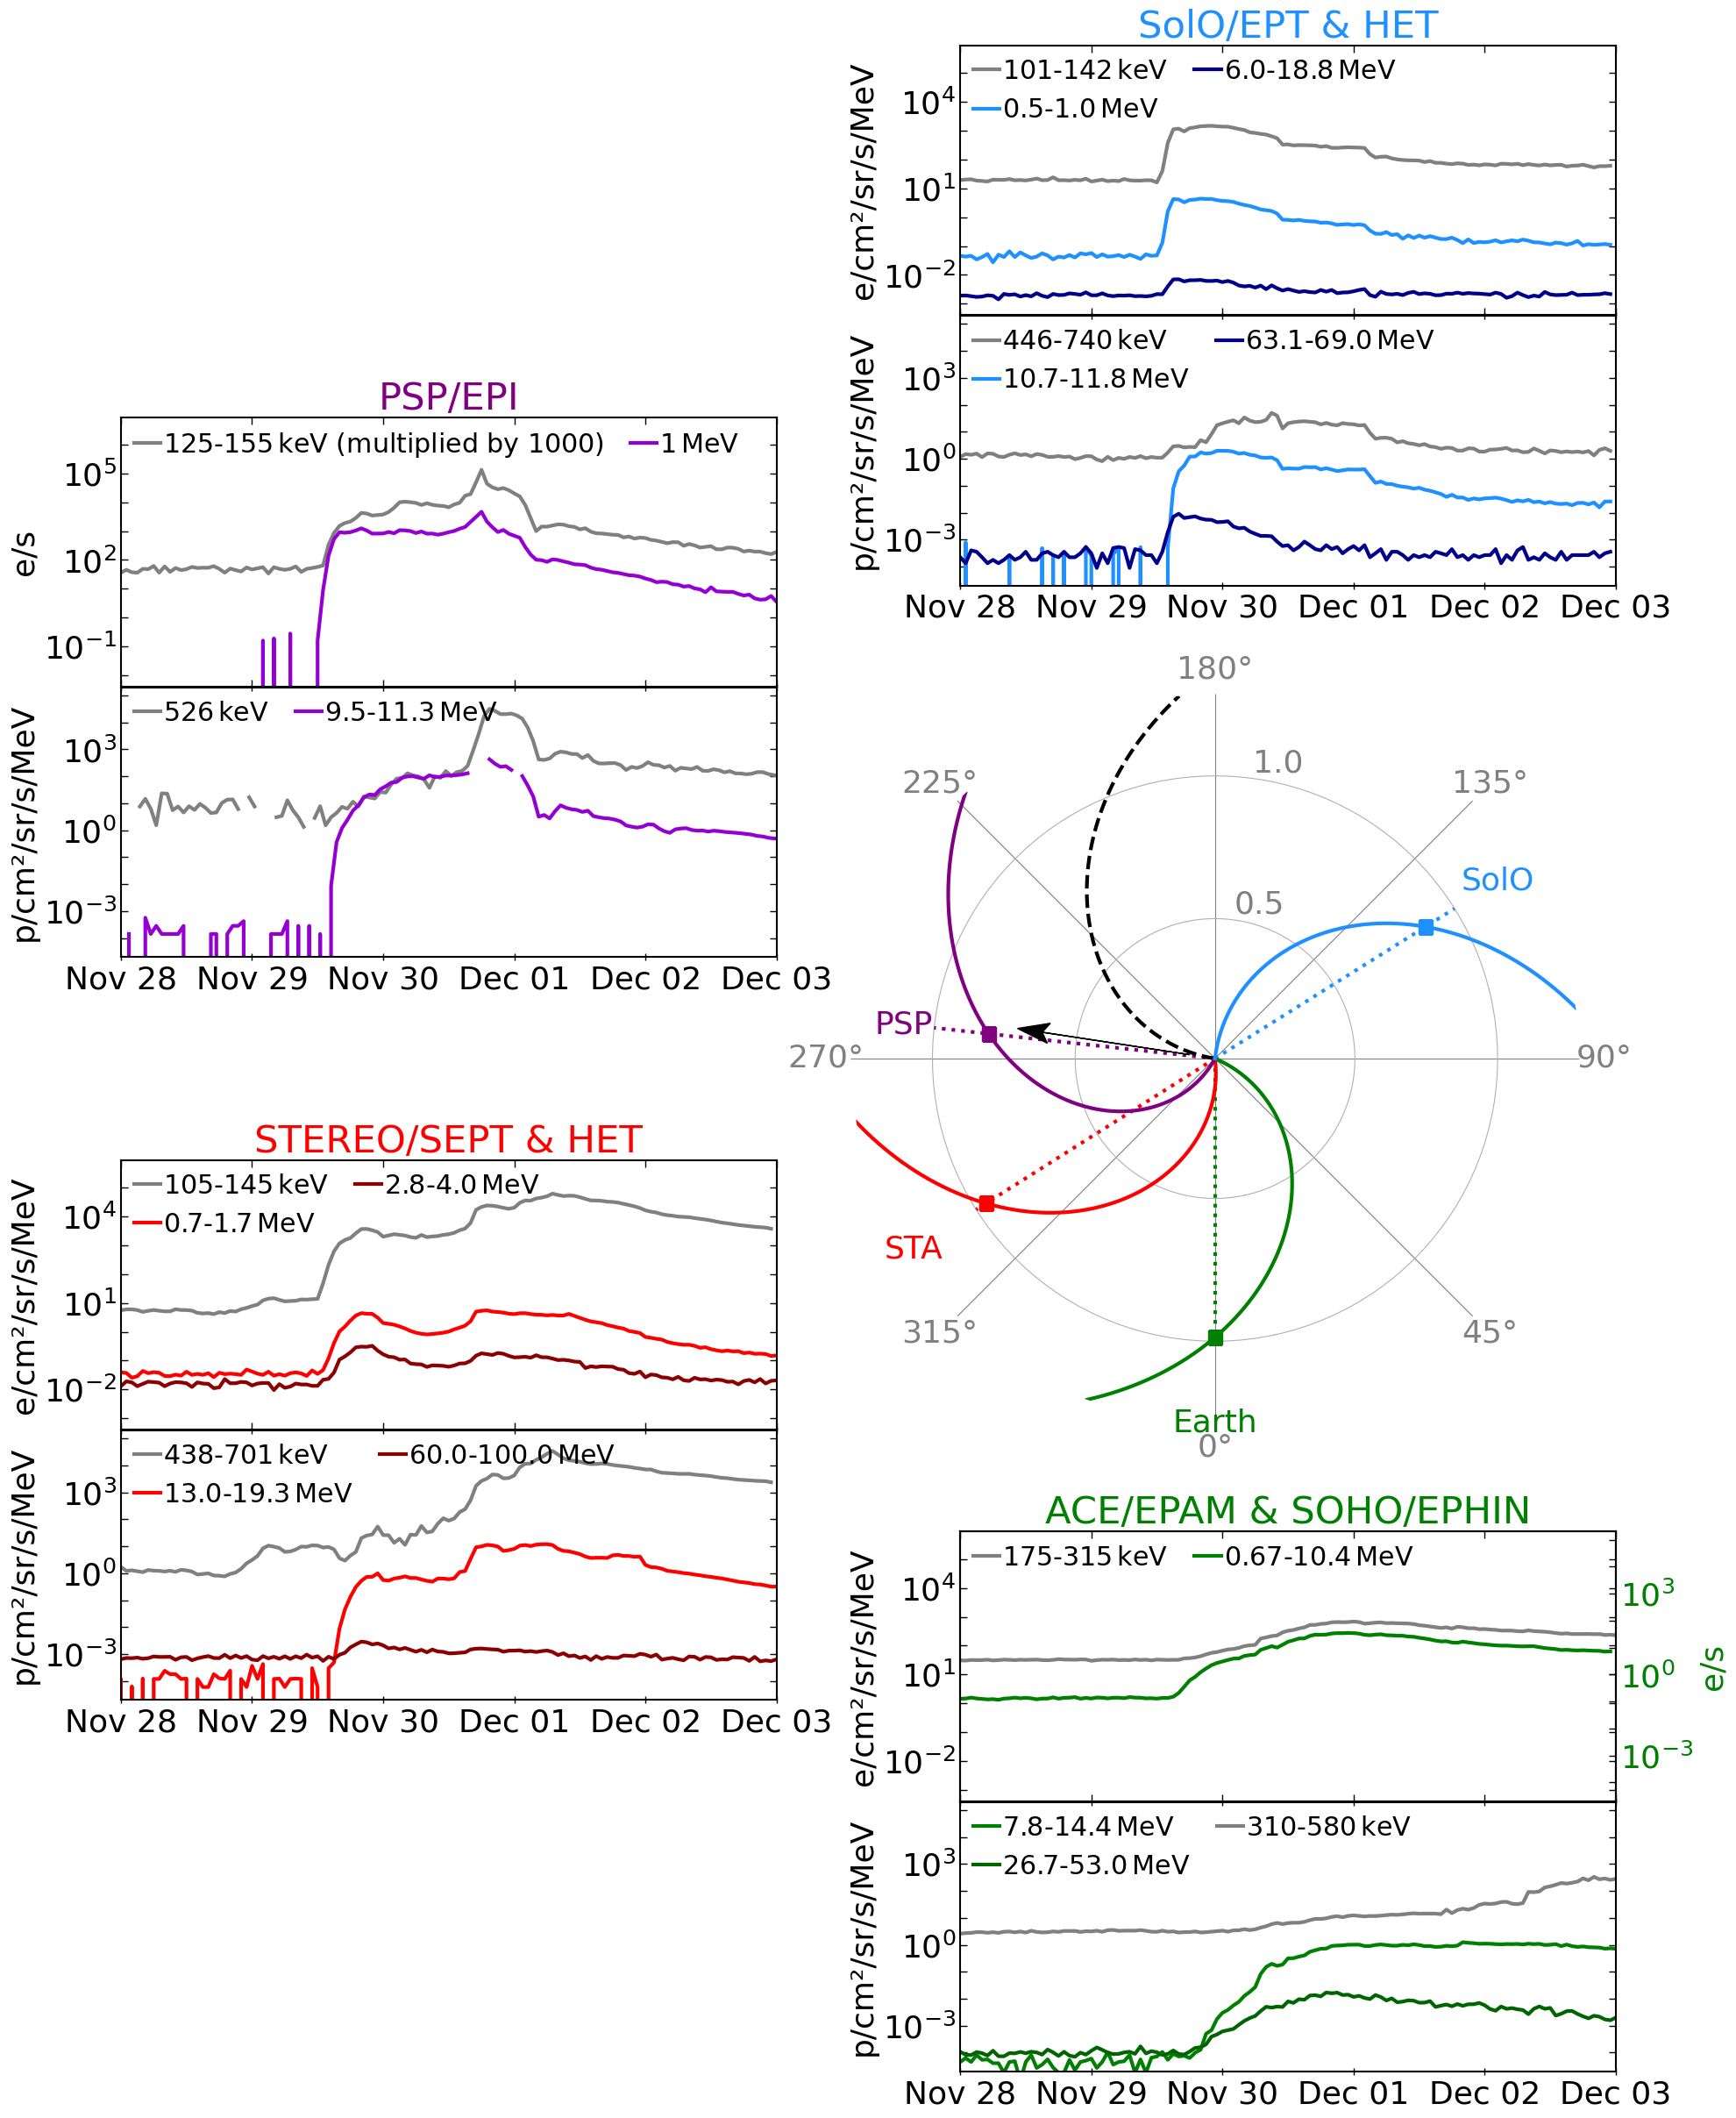
\includegraphics[width = 0.7\textwidth, height = 0.5\textheight]{images/2020-11-29_overview_plot.png}
	\caption[The first wide-spread \acl{SEP} event on Nov 29, 2020]{The first wide-spread \acl{SEP} event on Nov 29, 2020. The central panel illustrates locations of different spacecrafts and their magnetic connections to the Sun. Both proton and electron observations from \ac{SolO} (top), \ac{PSP} (top left), \ac{STEREO}-A (bottom left) and the Earth including \ac{ACE} and \ac{SOHO} are given. (Figure reproduced from \citet{Kollhoff-2021})}
	\label{Fig:SEP_widespread}
\end{figure}

The thorough explanations and summary of the remote-sensing observation of \acp{SEP} in radio, EUV, X-ray channels, particle injection and transport, composition, charge state, anisotropy and spectra evolution can be found in review papers \citep{reames2013two, Desai_Diacalone2016LRSP, Reames2021LNP}
Instead, in this part we briefly introduce the wide-spread \acp{SEP} and the multiple observation of \acp{SEP}.

Figure \ref{Fig:SEP_widespread} is the first widespread \ac{SEP} of the \ac{SC} 25 happened on 2020 November 29 that was observed by \ac{SolO} and also by \ac{PSP}, \ac{STEREO}, \acl{ACE} and \ac{SOHO} near the Earth, with a shift in the onset time \citep{Kolhoff2021AA, Kouloumvakos2022AA, Palmerio2022SpWea}. Both relativistic electons and higher energy protons with energy $>$50 MeV were observed. The particles in this event spread over a region 1 au spanning more than 230$^\circ$ longitude. This SEP is associated with an M4.4 class flare accompanied by a \ac{CME}, \ac{EUV} waves and type II/III radio bursts. The black arrow in the central panel indicates the location of the active region and the possible location of the central meridian of the \ac{CME}.  Depending on the magnetic connection between the \ac{CME}-driven shock and the instrument at different locations, as indicated by colored lines in central panel, the time profiles of particles have different shapes. For instance, \ac{PSP} and \ac{STEREO} connect closely to the central meridian, hence the intensity profile shape are similar to the \ac{SEP} we showed in Fig.~\ref{Fig:two_type_SEP}, i.e., abrupt increase with a later peak when the shock reached the spacecraft location. While Earth is about 166$^\circ$ away from the active region and is connectted to the western limb of the source, the intensity of the event slowly increases before they peak.

Recently, a comprohensive study of the second widespread \ac{SEP} of \ac{SC} 25 occured on 2021 April 17 has been carried out by \citet{dresing202317}. The particles were detected over a region of more than 210$^\circ$ longitude at six locations between 0.42 au and 1.62 au, including four used in the previous event, and \ac{Bepi} as well as Mars, though the Mars observation only provide a observational contrain. \citet{dresing202317} argued that the distinct SEP injections cover a wide range of longitudes might be responsible for this widespread SEP event.

As indicated from the above two examples, the wide spread \ac{SEP} event is a type of event that the particles can be spread over a large range in longitude ($>$ 200$^\circ$) though the minimum requirement of the longitudinal seperation has not been well defined \citep{Dresing_2014phd}. The shape of particle's temperal profiles at different locations, especially if they are far away from each others, varies a lot, which indicate possiblely completely different transport effect and source of particles. 
Therefore, one of the most important questions about wide spread \ac{SEP} is how the energetic particle spread through the heliosphere in such large longitudinal regions. Many ideas have been proposed to explain the longitudinal property \citep{Richardson2014SoPh, Dresing2012SoPh,Desai_Diacalone2016LRSP, Reames2021LNP}. The possible mechanisms of the large spread SEPs include:
\begin{itemize}
	\item Magnetic connection to an expanding coronal and IP shock \citep{Cliver1995ICRC, Torsti1999JGR, Reames1999, cane2003two, Richardson2014SoPh, Kouloumvakos2019ApJ}: 
	%The generally accepted reason for 
	The wide-spread energetic protons and heavier ions are accelerated in the shocks and are released from different shock fronts when they are connectted to the magnetic footpoint of the observer. Hence the \ac{SEP} distribution depends on the extend of the shock in the inner heliosphere.

	\item Cross-field diffusion \citep{Dresing2012SoPh}: The particles perpendicularly transport in the solar wind, which is a slow process compared with parallel transport along the magnetic field lines.
	
	\item Coronal transport \citep{Reinhard1974SoPh, Newkirk1978JGR}: This process spread energetic particles from the source region i.e. a flare or an acitve region, to the remote longitudes in the corona via a divergent magnetic field. 

	\item Multiple particle injections from different sources \citep{dresing202317}: The distinct \ac{SEP} injections covering a wide range of longitudes might be responsible for the widespread \ac{SEP} event.

	\item \ac{EUV} waves \citep{Rouillard2012ApJ, Park2013ApJ}:\ac{EUV} waves are large scale disturbances in \ac{EUV} images. Those waves encounter the magnetic foot point on the solar surface when they are propagating and expanding outward, which might be used to account for the wide spread \ac{SEP} events.
	\item Meandering magnetic field lines \citep{Laitinen2016AA, Laitinen2023ApJL}: The meandering walk of magnetic field lines is associated with turbulences in the solar wind and causes effecient particle movement across the magnetic field lines.
	\item Particle transport to remote longitudes by large-scale magnetic loops \citep{Klassen2018AA, Schrijver2013ApJ} and along the heliospheric current sheet \citep{Battarbee2018ApJ}.
	\item Mixture of the processes above.
\end{itemize}

To further clarify the processes leading to wide spread events, multi-spacecraft observations are essential for determining the properties of widespread \ac{SEP} events \citep{Kolhoff2021AA}. Previously, major contributions to understanding these events have been made by the combined measurements of \ac{STEREO} mission with its two spacecrafts, and the remote-sensing and in-situ measurements near \ac{L1}. Nowadays, with the new era of spacecraft, including \acl{PSP} \citep{Fox2016SSRv}, \acl{SolO}  \citep{Mueller-2020-SolO}, and the \acl{LND} \citep{Wimmer2020SSRv} we have a better oppurtunity to investigate the spectral variation, acceleration, transport processes and other aspects of wide spread \ac{SEP} events in more detail.

%In the above two example, we have already use multiple instrument to study the \ac{SEP} events. While the history of multiple observation dates back to 

%Nowadays, more and more space-born telescopes have been developed and launched to study the center of our heliosphere and moniter the variation of the plasma environment.  
%Study both in-situ and remote.
%Now - \ac{SOLO} \ac{PSP} and \ac{Bepi},  Mars, STEREO missson, helios mission, new mission from China, \citet{Wang2020Solarring,}India

%A numerous observation and simulation studies have been carried on in the past few decade since the discovery of SEP back to 1950s. The major questions of SEP focus on the origin, acceleration and transport of those high energy particles.\citep{Desai_Diacalone2016LRSP}, which is also the goal of recently two missions \ac{PSP} and \ac{SolO}. 

%=========================================

\section{Galactic cosmic rays}

\begin{figure}[htb]
	\centering
	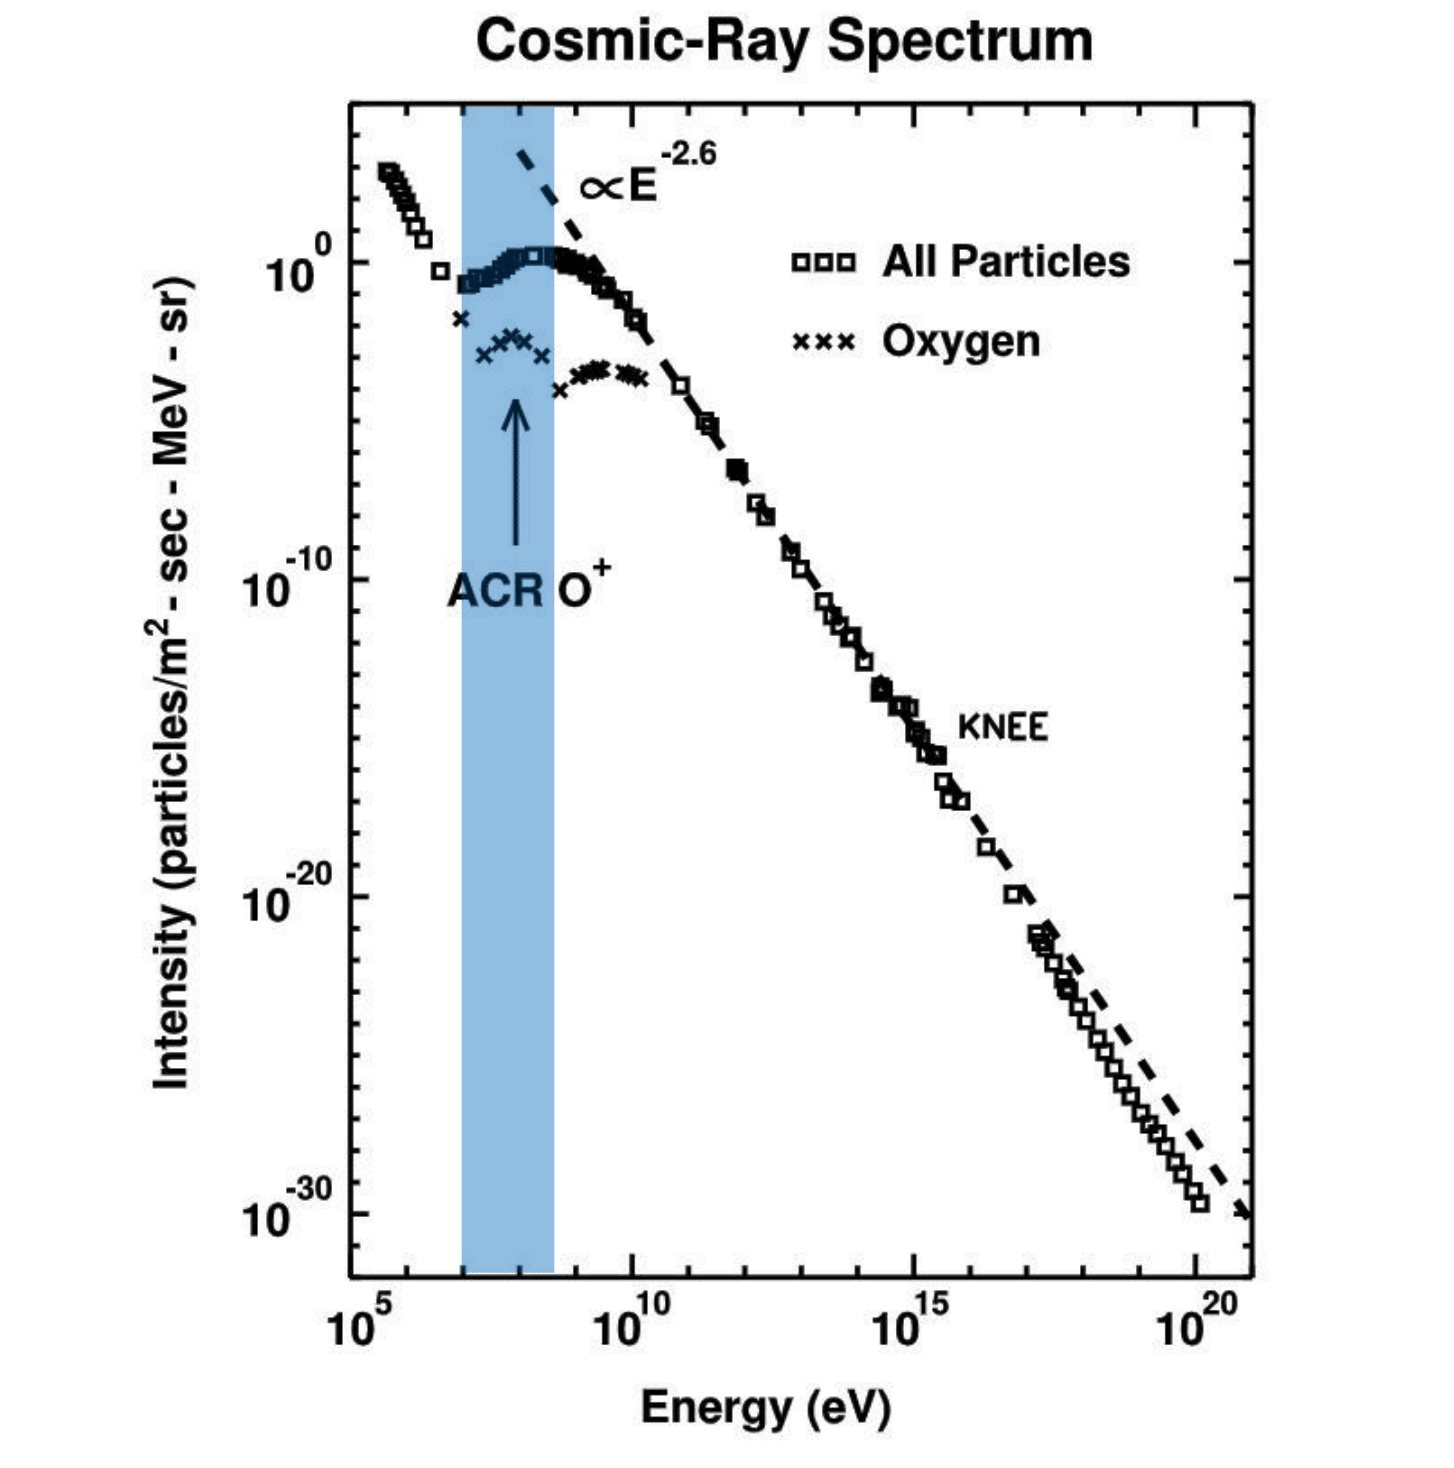
\includegraphics[width = 0.7\textwidth]{images/gcr_spectra_shadow.png}
	\caption[The cosmic-ray spectrum of all particles at 1 au]{The cosmic-ray spectrum of all particles and \ac{ACR} oxygens observed at 1 au. This figure is reproduced from \citet{Giacalone2022SSRv, Giacalone2012SSRv}, which is originally from \citet{Jokipii1990AIPC}.
	The spectrum is plotted in more than 15 orders of magnitude on the energy scale and about 30 orders of magnitude on the intensity scale. In particular, it extends the high energy end of Fig.\ref{Fig:Oxygen_spectra_heliosphere}.}
	\label{Fig:Oxygen_spectra_cosmic_ray}
\end{figure}
%\url{https://timeline.web.cern.ch/victor-hess-discovers-cosmic-rays-0}
The first discovery of \acp{GCR} was made by the Victor Hess in 1912 when he carried out a ballon experiement. The initial purpose of the experiement was to find the source of ionizing radiation in Earth's atmosphere using an electroscope. However, as the ballon climb-up during the experiment, he found that the ionization rate measured in the electroscope showed less significant decrease than anticipated. Such a discrepancy was attributed to the existence of cosmic rays which increase the radiation in the atmosphere.

Figure \ref{Fig:Oxygen_spectra_cosmic_ray} show the spectrum of all cosmic ray particles that could be observed at 1 au. This spectrum includes both the \ac{ACR} and \ac{GCR} components. The \acp{GCR} are indicated as empty squares. In the right half of the spectra with energy above 1 GeV, the spectrum could be simply fitted by power a law spectrum with an index of about -2.6. The higher energy knee in the \ac{GCR} spectrum is around few PeV energy and reflects the dominant contribution of hypernovae \citep{Sveshnikova2003AA, Hoerandel2003APh}. The lower energy spectrum  below 1 GeV is shown as a "turn over" structure which is more complicated and could not be fitted by a signel power law. 

\acp{GCR} consists of multiple energetic particle species spanning a wide range of energy, which are mostly simple protons, about 89\% and the remains are shared by 9\% helium nuclei, a small fraction of neuclei of heavier elements (1\%) and 1\% electrons. %, positron and antiproton.
It is believed that \acp{GCR} mainly originate from the supernova remanents which are at distant locations away from the Sun \citep{Blasi2013AARv2013,Bhattacarjee2000PhR,Fermi1949PhRv}. Particles obtain the energy from the shock waves which are generated during the explosion of supernova \citep{blandford1978particle}.
%When the shock wave travel through the surrounding interstellar gas, the kinetic energy of shock are tranfer to the  (neutral gas?) by the (Fermi-acceleration, ciataion and the acceleration process), Utilimatly, the energetic particle with energy up to 10$^12$ eV are created.

After a long travel, \acp{GCR} arrived at the very local bubble which is controlled by the Sun and its magnetic field, i.e. our heliosphere.
Before entering the heliosphere, the particles are assumed to be isotropic in the space and are slowly varying in time. Because cosmic rays are fully charged, they are deflected by the magnetic field when they propagate towards the heliosphere and the directions of those particle are normalized by the strong magnetic field. Hence when they arrived at the space outside of our heliosphere, we obtained an nearly isotropic and constant intensity profile of \ac{GCR}, which are the \ac{LIS} or the heliospause spectra, as observed by the Voyager missions after they crossed the boundary of solar system and entered the interstellar medium \citep{Stone2013Sci, Cummings2016ApJ,Stone2019NatAs}.
%is the so-called \ac{LIS}.

%\ac{LIS} are assumed to be the input spectra at the modulation boundary and will be modulated as a function of the position, energy, and time after cosmic rays diffuse into the heliosphere. The lower energy part of \ac{LIS} have been observed by the voyoger missions after they crossed the boundary of solar system and entered the interstellar medium \citep{Stone2013Sci, Cummings2016ApJ,Stone2019NatAs}.

%To model the solar modulation on the particle transportation of GCR spectra, an input particle spectra need to be specifield, which is the so-call LSTM [citaion of LSTM].

When propagating in the heliosphere, cosmic rays are modulated by the solar wind emitted from the Sun and its embedding magnetic field periodcally. The relavant process of the solar modulation could be described by a basic \ac{TPE} which is first derived by \citet{Parker1965Pss}. The same equation was also derived by \citet{Gleeson1967ApJ} in a more rigorous way. This equation is based on the motion of charged particle in the frequently changing magnetic field and averaged over the pitch angle of particles moving in the magnetic field. The precondition of this equation is the reasonable assumption of the isotropically distributed \acp{GCR}. The \ac{TPE} gives the phase-space distribution function, $f$ as the function of position, time and momentum magnetitude. In \citet{Potgieter2013LRSP}, the helispheric \ac{TPE} is rewritten in the following form:

	\begin{equation}
		\underbrace{\frac{\partial f}{\partial t}}_{a} = - ( \underbrace{\boldsymbol{V}}_{b} + \underbrace{\langle v_d \rangle }_{c}) \cdot \nabla f + \underbrace{\nabla \cdot (\boldsymbol{K_s \cdot \nabla f})}_{d} + \underbrace{\frac{1}{3}(\nabla \cdot \boldsymbol{V}) \frac{\partial f}{\partial ln P}}_{e}
		\label{Eq:Transportation_equation}
	\end{equation}

where $f(r, P, t)$ is the cosmic ray distribution as the function of the time t, particle rigidity P and 3-dimensional position in space. Compared with the $\sim$ 11  and 22 years solar activity cycle, the periodcal solar rotation ($\sim$ 27 days) and  the time of the solar wind traveling to the edge of heliosphere ($\gtrsim$ 1 years) are short-term variations. Hence the steady-state solution with  $\frac{\partial f}{\partial t} = 0$ (part a of Eq.\ref{Eq:Transportation_equation}) is a reasonable assumption and considered when we study the solar modulation of the cosmic ray. Terms on the right side of the Equation \ref{Eq:Transportation_equation} include four effects that are used to describe the variation of the cosmic rays: (b) convection due to the solar wind velocity $\boldsymbol{V}$; (c) drift effects caused by the gradient and curvature of the large-scale \ac{HMF}, which is estimated by a 3D Archimedean spiral \citep{Parker-1958}, $\langle v_d \rangle$ represents the averaged drift velocity; (d) diffusion effects caused by the turbulent magnetic field, with $\boldsymbol{K}_s$ the symmetrical diffusion tensor; (e) adiabatic energy change and deceleration due to the expansion of the solar wind. 

\ac{TPE} is a highly non-linear partial differential equation. A simplified solution of the \ac{GCR} spectra called \ac{FFS} was first derived by \citet{Gleeson1967ApJ, Gleeson1968ApJ}. The solution simply depends on the kinetic energy $T$ of particles and the solar modulation potential. Later, reasonable \ac{GCR} spectra of the particle with energy above 150 MeV were given by \citet{Gleeson1973ApSS}.
With the development of computer technques and numerical studies, simulations are becoming more and more important in studying the tranport and solar modulation of the cosmic rays \citep{Jokipii1979ApJ, LeRoux1995ApJ, Manuel2011AdSpR, Potgieter2013LRSP, Vos2015ApJ, Vos2016SoPh,Boschini2019AdSpR, Boschini2022AdSpR, 
Corti2019ApJ, Shen2019ApJ}. 
Commonly used \ac{GCR} models like Badhwar-O'Neill \citep{Oneill2006AdSpR,ONeill2015, Slaba2020SpWea}, CREME \citep{Tylka1997ITNS,Weller2010ITNS} and HELMOD \citep{Boschini2018AdSpR} with the solar modulation and sunspot number as input could reproduce the GCR intensity and spectra. The model predictions are consistent with the measurements from \ac{ACE} at 1 au and the Voyager probes in different regions of the helisophere \citep{Boschini2019AdSpR}.

\begin{figure}[!htb]
	\centering
	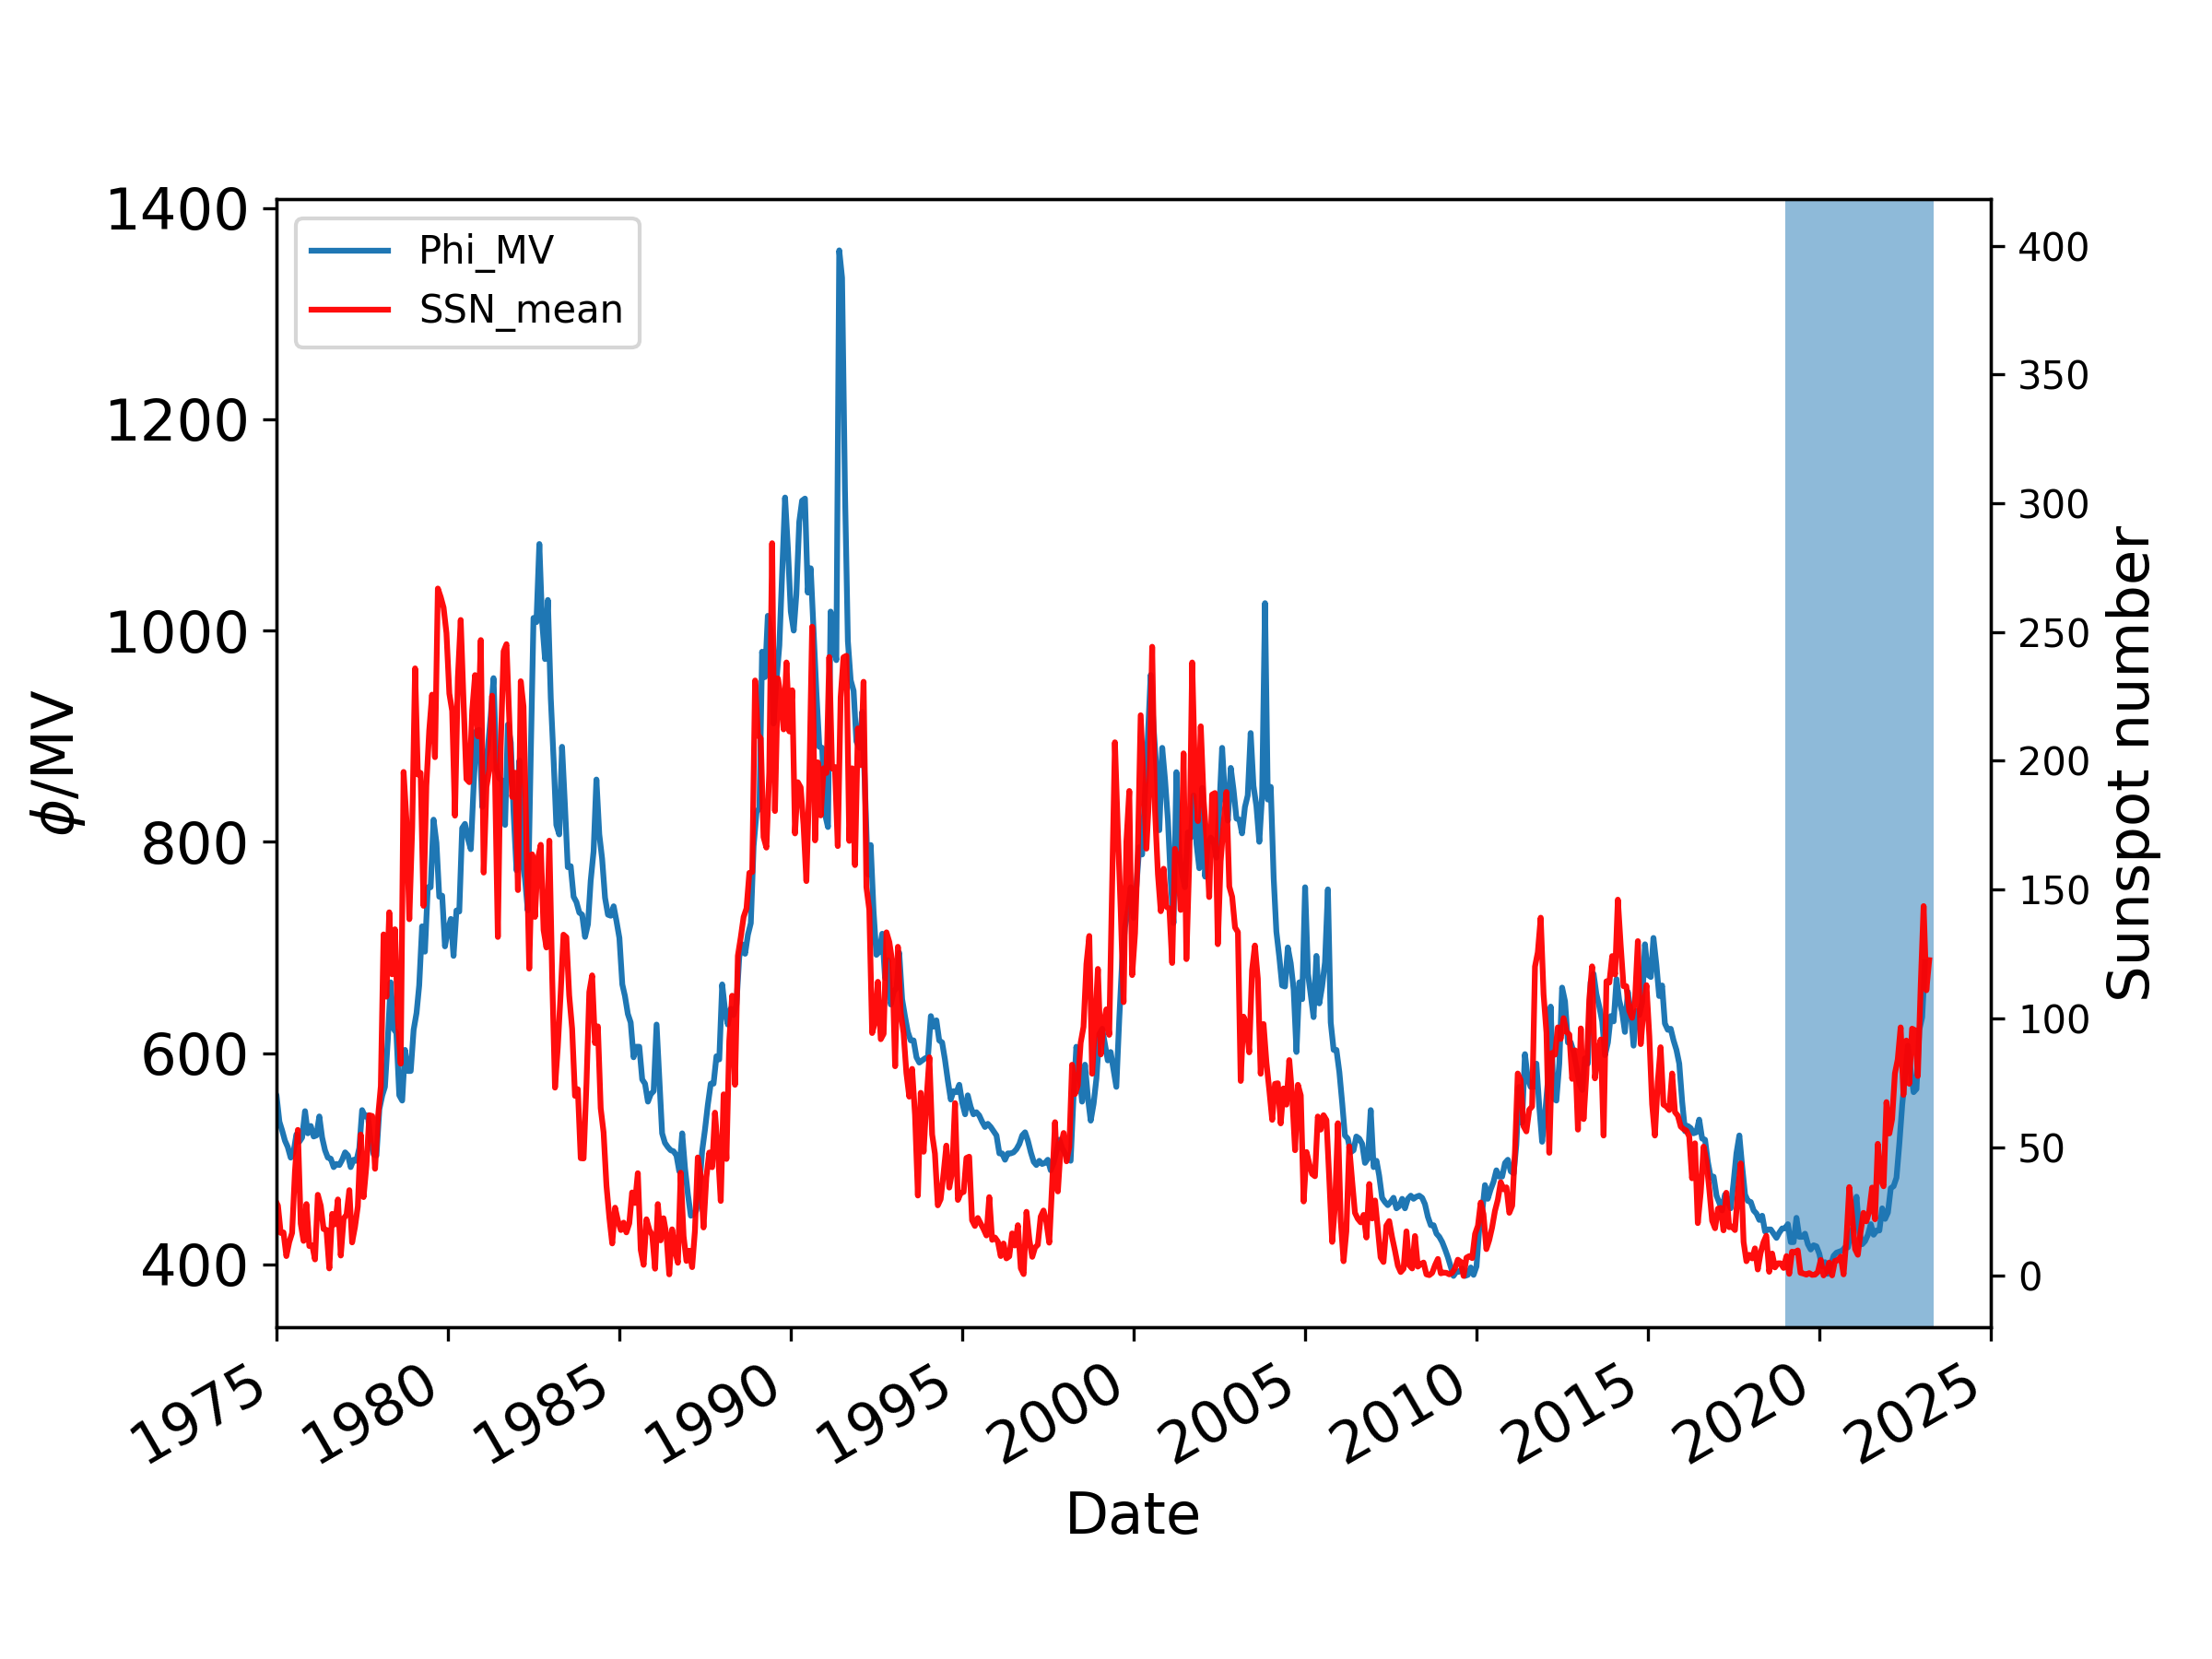
\includegraphics[width = 0.9\textwidth]{images/Solar_modulation.png}
	\caption[Sunspot number and Neutron monitor count data]{Oulu neutron monitor count rate downlowded from the \ac{NMDB} measured by the Sodankyla Geophysical Observatory of the University of Oulu, Finland and the monthly averaged sunspot number from Solar Influences Data analysis Center (SIDC), Royal Observatory of Belgium, Brussels. The period that we are interested in is marked by the blue shaded region.}
	\label{Fig:Solar_modulation}
\end{figure}
%\footnotetext{\url{https://www.nmdb.eu/data/}}
%\footnotetext{\url{https://www.sidc.be/silso/datafiles}}

%The solar modulation potential ($\phi$) \cite{Usoskin 2011}, data are downloaded from \url{https://cosmicrays.oulu.fi/phi/phi.html}, 

Figure \ref{Fig:Solar_modulation} shows the monthly averaged sunspot number since 1975 in red and the Oulu neutron monitor count rate in blue.
%the solar modulation potential ($\phi$) \cite{Usoskin 2011}.
Sunspot number is a proxy for the solar activity. While the neutron monitor registers neutrons that generated when high-energy charged particles strike and penetrate the Earth's atmosphere. The overall variation of the neutron monitor count rate is anti-correlated with the averaged sunspot number.
The count rate peaks when the sunspot number is minimum during the solar activity minimum and vice versa in the solar activity maximum. The time between two neighbouring solar minima is about 11 years, which is the period of the solar activity cycle and caused by the polarity reversal of the solar magnetic field.

Besides the magnetic field reversal, drift effects play an important role in the 22-year cycle of the cosmic ray intensity \citep{Jokipii1977ApJ}. Such effects are clearly observed in the temperoal variations in Fig.~\ref{Fig:Solar_modulation}.
During the negative polarity (donated by A $<$ 0) cycle, \acp{GCR} have a more peaked time profile than the positive polarity (donated by A $>$ 0) cycle, which have a plateau-like profile. 
This is because in the negative magnetic polarity cycle, the positively (negatively) charged particles drift inwards (outwards) mainly along the equatorial plane in the heliosphere and drift outward (inwards) through the open magnetic field line in the polar region which results in a sharp change of the intensity. While in the positive polarity cycle, the drift direction of the particles is opposite to that in negative cycle which causes the plateau region on the solar minimum. Fig.~\ref{Fig:drift_effect} illustrates the drift effects in the opposite polarity cycles, specifically depicting the drift directions of the positively charged particles such as helium, oxygen.

\begin{figure}
	\centering
	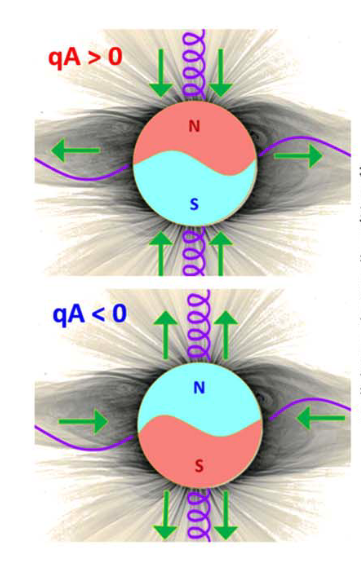
\includegraphics[width = 0.4\textwidth]{images/drift_effect.png}
	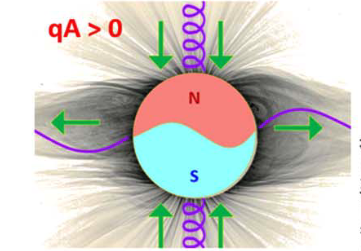
\includegraphics[width = 0.4\textwidth]{images/drift_effect_2.png}
	\caption[The gloabl drift pattern of positively charged particles in different polarity]{The illustrations of the cosmic ray drift pattern in negative polarity (left) and positive polarity (right). The north pole of the Sun has a positive magnetic field, while the south pole has a negative magnetic field during the A $>$ 0 cycle. The signs of the magnetic field in the south and north pole are reversed during the A $<$ 0 cycle. The green arrows indicate the drift directions of ions and the wavy lines in purple are the heliosphere current sheets. This figure is adapted from the Fig. 4 of \citep{Rankin2022ApJ}}
	\label{Fig:drift_effect}	
\end{figure}

Furthermore, the drift effects which depend on the charge sign of particles and the magnetic polarity are also reflected in the spatial gradient of the cosmic rays, including both \acp{GCR} and \acp{ACR}. In the following, we recap the observation of \ac{GCR} particles spatial gradient with energy above hundreds MeV/nuc, although those observations are not the focus of this thesis. The details of the \ac{ACR} component are discussed in the next section.

An evidence of \ac{GCR} latitudinal variation is the observation from Ulysses. \citet{Simpson1995GeoRL, Heber1996GeoRL, Heber1996AA} determined positive variations with an upper limit of 0.25 \% /$^\circ$  in the A $>$ 0 solar cycle. When the polarity changes to the negative sign, the latitudinal gradient was found to change the sign accordingly and decrease to a very small value with a maximum of -0.1 \%/$^\circ$ \citep{desimone2011ASTRA, Gieseler2016AA}. It was also found that the solar modulation conditions in the same solar polarity but different solar cycle could affect the latitudinal gradient \citep{Gieseler2016AA, Vos2016SoPh}. Moreover, the latitudinal gradient of electron was first determined by \citet{Heber2008ApJ}, which was about 0.2 \% /$^\circ$ and agreed with the proton gradient.

Recently, by revisiting \ac{GCR} proton data from Helios E6, \citet{Marquardt2019AA} found that the radial gradient in the inner heliosphere (0.3 - 1 au) is about 6.6 $\pm$ 4 \% /au, compared with the previous results of 2.5 $\pm$ 0.5 \% /au between 2 and 28 au \citep{Webber1981JGR}. Such a discrepancy indicates that the radial gradients in the inner helioshphere have different behavior than those in the outer heliosphere.

%The spatial gradient, including the latitude and radial gradients have already been observed by multiple missions for the region from 1 AU to the edge of the heliosphere in the past few solar cycles, for instance the two Voyager probes, the Ulysses spacecraft, Pioneer and also combined the measurements like PAMELA from L1 point, [citaion]

\section{Anomalous Cosmic Ray}

\acp{ACR} are mostly the singly charged energetic particles dominantly in the energy range between few meV/nuc and $\sim$ 100 MeV/nuc. \acp{ACR} were first discovered with \ac{IMP} 7 and 8 missons, which date back to 1970s \citep{Garcia1973ICRC, Hoverstadt1973PhRvL, McDonald1974ApJ}. By analyzing the low energy spectra of cosmic rays, scientists found "unusual" enhancements of the flux of helium ($<$ 50 MeV/nuc), oxygen and nitrogen ($<$ 20 MeV/nuc) below 100 MeV/nuc. As the oxygen spectrum which is pointed out by an arrow in Figure \ref{Fig:Oxygen_spectra_cosmic_ray} show, the intensity of lower energy oxygen does not decrease as the energy decreases from hundred MeV/nuc to MeV/nuc, as expected from our understanding of the \ac{GCR} spectrum, but increases instead. Those particles have been known as \acp{ACR}. \ac{ACR} elements include helium, nitrogen, oxygen, and neon that have been discovered in the inner heliosphere, and Ar and possibly protons that have been found in the outer region of heliosphere \citep{Klecker1995SSRv}.

One of the key chararcteristics of \acp{ACR} is their singly charged nature \citep{Klecker1980GeoRL,Adams1991ApJ, Klecker1995ApJ}. This property suggests a distinct source for \acp{ACR} and seperate it from \ac{GCR} and \acp{SEP}, as well as limits the travel time of \acp{ACR} in the space. Direct measurement of the charge states of ten of MeV/nuc particles is challenging with the current measurement techniques. Therefore, in the early stage, most studies relied on the propagtion model to infer the charge states. For example, \citet{Klecker1980GeoRL} reported that the \ac{ACR} oxygen have lower charge states of $<$ 3 by observing the phase leg effect. Later, a clever approach using the Earth's magnetic field as the magnetic spectrometer was employed to determine the charge states. \citet{Adams1991ApJ} and \citet{Klecker1995ApJ} both confirmed the charge states of oxygen, nitrogen and neons on the energy of tens of MeV/nuc, which were found to be equal to 1.

It is widely believed that \acp{ACR} are the high energy interstellar pick-up ions which are accelerated in termination shock of the heliosphere \citep{Fisk1974ApJ}. These pick-up ions originate from interstellar neutral atoms, which are ionzied by the solar \ac{UV} and charge exchange with the solar wind when those atoms drift into the heliosphere. Once ionized, solar wind picks them up and transports them to the outer heliosphere, where pick-up ions are accelerated by the blunt termination shocks \citep{McComas2006GeoRL} and acquire energies of several tens of MeV/nuc. Termination shock as the origin of \ac{ACR} is one of the mostly accepted theory and supported by observations of various instruments \citep{McComas2019ApJ, Cummings2019ICRC}. 

As aforementioned and explained, the transport of cosmic rays in the heliosphere can be described by the \ac{TPE} equation. Various processes are modeled in that equation including diffusion driven by the \ac{HMF} fluctuation, adiabatic energy loss, convection in the expanding solar wind and the drift effects in the large-scale \ac{HMF} which have already been successfully modeled \citep{Parker1965Pss, Jokipii1977ApJ, Jokipii1981ApJ}.

At 1 AU, similar to \acp{GCR}, the intensities of \acp{ACR} are heavily modulated as they traverse the solar wind and globar \ac{HMF}. Figure \ref{Fig:ACR_solarmodulation} illustrates the comparison between the \ac{ACR} oxygen intensity and the Newark neutron monitor count rate which serves as a proxy of the \acp{GCR} variation in the deep space. The \acp{ACR} intensities show clearly the peaked and plateau-shaped profiles which depend on the magnetic polarity over the last two and a half solar cycles. In particular, during periods of negative magnetic polarity, ions drift into the heliosphere near the equatorial region along the \ac{HCS} but drift outward from the region near the south and north pole. The opposite behavior occurs during the positive polarity \acl{SC}.

%Such a trend is consistent with \ac{GCR} and neutron monitor 
%measurement.


\begin{figure}
	\centering
	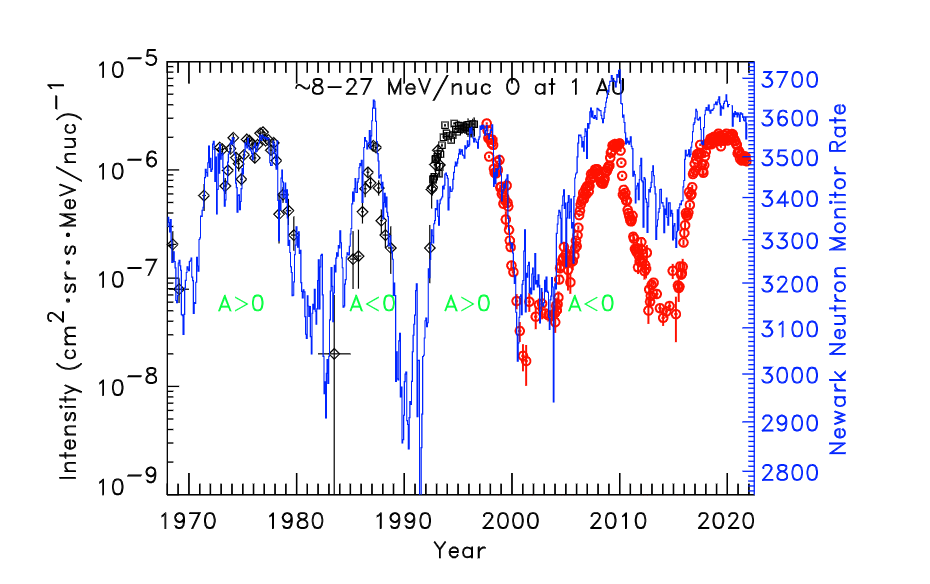
\includegraphics[width = 0.9\textwidth]{images/ACR_solarmodulation.png}
	\caption[Long term variation of \ac{ACR} oxygen and neutron monitor count rate]{ACR oxygen intensity variation with energy between 8 and 27 MeV/nuc at 1 AU measured by ACE/SIS instrument (red) and count rate of Newark Neutron monitor (blue). The blue data points are from the earlier measurements \citep{Mewaldt1993GeoRL}. (Figure reproduced from Figure 6 of \citet{Giacalone2022SSRv})}.
	\label{Fig:ACR_solarmodulation}
\end{figure}


As discussed previously, the spatial distribution of \acp{ACR} along the radial and latitudinal direction contains valuable insight into how the particles transport and being accelerated throughout the helioshphere \citep{Rankin2021ApJ}. By quantifying the magnitude of this gradient, we can estimate and reconstruct the transport processes involving drift and diffusion of \acp{ACR} in the heliosphere. The following general equation is used to model the radial and latitudinal gradients:

\begin{equation}
	\mathrm{ln}(\frac{f_{M}}{f_{E}}) = G_r \Delta R  + G_{\theta} \Delta \theta + C
\end{equation}
where $f_{M}$ is the particle flux measured by spacecraft located away from 1 au and the equatorial plane, like \ac{SolO}, \ac{PSP}. On the other hand, $f_{E}$ is the flux measured at 1 AU by space missions like \ac{SOHO}, \ac{ACE}; $G_r$ and $G_{\theta}$ are the radial and latitudinal gradients, respectively. $C$ is a constant term to account for any additional contributions.

%%% TO DO: list a table of the radial and latitudinal gradient of ACRs case. I already get confused for the sign of the gradient. and polarity

As predicted from the cosmic ray transport model, the latitudinal gradient changes sign from positive to negative or vice versa during different polarity \ac{SC}. The evidence of the change-sign nature of latitudinal gradient in the outer heliosphere were first determined by the two Pioneer and Voyager missions \citep{Mckibben1979ApJ, Cummings1987GeoRL, Christon1986JGR}. They found that latitudinal gradients of 15 Mev/nuc \ac{ACR} helium during \ac{SC} of A $>$ 0 range from 2.1 to 3.1\% /$^\circ$. In contrast, during A$<$0 \ac{SC} the gradients varied between -2.2 and -1.6 \% /$^\circ$. Moreover, \ac{ACR} oxygen exhibited an even larger latitudinal gradient ranging from -3.7 to -2.9\%/$^\circ$ \citep{Cummings1987GeoRL}.

The Ulysses mission, operating in the inner heliosphere (below 5 au), significantly expanded our understanding of cosmic rays by providing the polar region measurements, thus covering a wider latitude region up to 80$^\circ$. \citet{Lanzerotti1995GeoRL} and \citet{Heber1998JGR} conducted studies during the positive polarity period and found the latitudinal gradients varying between 0.39\%/$^\circ$ and 2.12 \%/$^\circ$. However, during the opposite solar polarity period, the respective gradients were reduced by approximately five times to about -0.3 - 0.4 \% /$^\circ$, which is consistent with zero. \citet{Cummings2009GeoRL} concluded that particles could not drift into the inner heliosphere along the \ac{HCS} in this solar cycle. In addition, a north-south asymmetry of cosmic rays was reported by \citep{Simpson1996ApJ}.

Studies investigating the radial gradients of \acp{ACR} are still ongoing and discrepancies have been found between the recent measurements in the inner heliosphere and the previous studies \citep{Webber1981JGR, Marsden1999AdSpR}. Recent studies by \citet{Rankin2021ApJ, Rankin2022ApJ, Marquardt2018AA}, utilizing different measurements from Helios and \ac{PSP}, have reported a consistent ACR oxygen radial gradient about 45\% /au during A $>$ 0 solar cycle. However this gradient is approximately three times higher than the measurement reported by \citet{Webber1981JGR}. Moreover, \citet{Rankin2022ApJ} reported the radial gradient of ACR helium with energies between 4 - 45 MeV/nuc during the last solar activity minimum (2018-2020), which was estimated to be approximately 25$\pm$ 5\% /au. Those values are also higher than the prior observations from Pioneer, Voyager and Ulysses mission \citep{McDonald2001ICRC, Webber1981JGR, McKibben1989JGR, McDonald1986GeoRL, Cummings1987GeoRL, Cummings1995GeoRL}. The discrepancies observed in the radial gradient of \acp{ACR} are still worth  further investigating, particularly with the new measurements from \ac{SolO} and \ac{PSP} which are operating below 1 au.


\section{Radiation hazard of energetic particles}


High-energy particles pose a significant threat to the human body and electronic hardwares in the deep space and on the surfaces of solar system bodies, such as Mars and Moon, where effective protection from the atmosphere and an inner magnetic field is absent.
These particles have the ability to damage the \ac{DNA} in our cells when they penetrate tissue or organs, even leading to cell death.
High doses of radiation caused by high-energy charged particle or neutral parrticle result in \ac{ARS} or \ac{CRI}, which are rapid whole-body responses \footnote{\url{https://www.nrc.gov/about-nrc/radiation/health-effects/high-rad-doses.html}}. Furthermore, prolonged exposure to the radiation environment increases the risk of cancer, even after the mission is completed.

In addition to the health risks for astronauts, the high energy particle can also cause degradation and damage to instruments and the electronic systems onboard the satellite in space. One of primary reason of the instrument failure is due to the so-called \acp{SEE} which is the change of state of a memory cell or transistor in electronic devices, induced by ionizing particles, particularly heavy ions. \acp{SEE} can result in permanent or temporary failure of the electronic systems, potentially leading to the loss of mission. 


% https://www.epa.gov/radiation/radiation-health-effects

The radiation hazard posed by the energetic particles, based on their source, can be seperated into two types: short-term but intense radiation caused by \acp{SEP}, and prolonged but lower intensity radiation mainly caused by \acp{GCR}.
Exposure to intense radiation can lead to \ac{ARS}, such as nausea and vomiting. Chronic exposure to the \ac{GCR} radiation environment, although not fatal immediately, can increase the risk of late-term consequences, such as cancer, damage to the central nervous system and many other side effects \citep{Guo2021AARv_rad, cucinotta2006cancer, Kennedy2014LSSR, Iancu2018Frontiers}. 



Fig.~\ref{Fig:Rad_GCR_radiation} illustrates the variations in radiation dose rate on the surface of Mars over the last ten years. Several large \acp{SEP} with sufficient energy penetrated the atmosphere of Mars, resulting in an increased dose rate up to few times higher than the pre-event background. Apart from those abrupt enhancements, the overall dose calculated by the \ac{MSL}/\ac{RAD} shows an increasing trend from the solar activity maximum to the solar activity minimum during the \ac{SC} 24. This long term trend is due to the solar modulation on the \ac{GCR} intensity.
Therefore, understanding the variations in radiation dose rates is crucial for the assessment of potential health risks and to properly schedule human activities in outer space. 


Fig.~\ref{Fig:SEP-radiation_hazard} illustrates the spectra of two famous \ac{SEP} events that happened in April 1998 and September 1989. The colored regions indicate the proton energy that pose threats to human activities. Protons with energeis above 150 MeV (red) are considered as hard radiation, which can penetrate 20g/cm$^2$ of aluminium. Soft protons are categorized as particle with energies abve 50 MeV (shown in yellow), which are capable of penetrating spacesuits and the skin of spacecraft \citep{Reames2021LNP}. 

%secondary electrons produced in the athmsphere are also relevant (at least for Mars)
In addition to the radiation we discussed earlier, secondary particles such as protons and neutrals generated from the interaction between energetic paritcles and lunar regolith are another signicant contribution to the radiation dose. Secondary protons possess enough energy to penetrate space suites and cause radiation hazards \citep{Xu2022FrASS}. Secondary neutrals are even more detrimental than the charged particles due to their high penetrating ability and high biological effectiveness, despite their lower intensity.
\citet{Spence2013} estimated the amount of radiation hazard caused by \acp{GCR} and secondary particles on the lunar surface by conducting simulations and found that secondary particles account for 8.6\% of the overall radiation dose.

In the future, potential human missions may require longer stays of astronauts on the surface of solar system bodies or in space while traveling to their destination. As a result, the probability of exposure to the intense radiations and the risk of exposure to the chronic radiations are considerably increased. Properly estimating and understanding the radiation hazard in different situations and locations is crucial for preparing for future human missions.



%Apollo mission not affected by the SEP, 


%Earth is protected by atmosphere and magnetosphere
%Mar not, Lunar not.


\begin{figure}
	\centering
	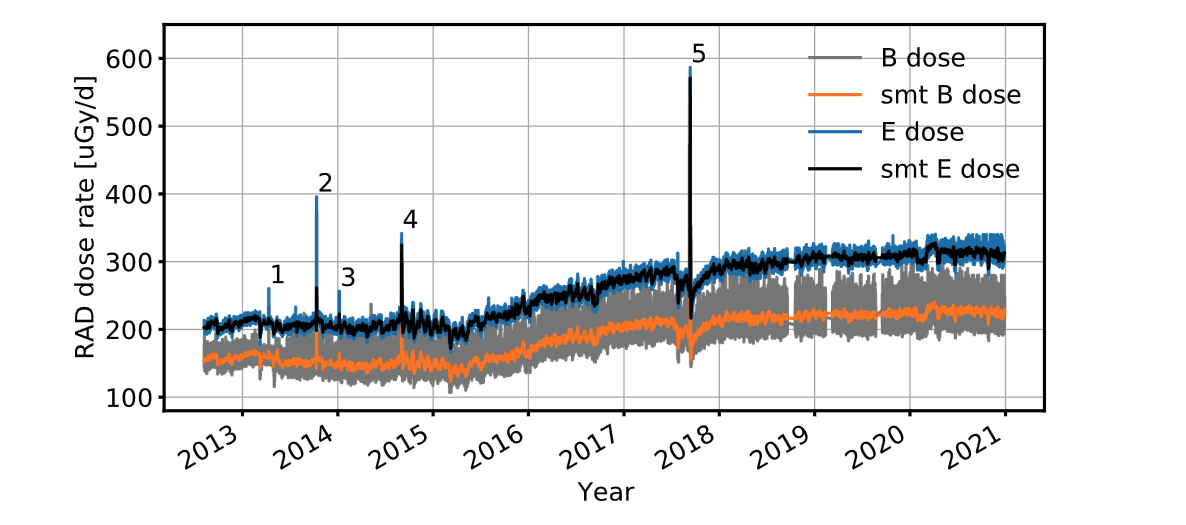
\includegraphics[width = 0.9\textwidth]{images/Rad_GCR_radiation.png}
	\caption[The long term radiation dose rates on the Martian surface]{The radiation dose rates on the Martian surface, measured by \ac{RAD} in the silicon detector B (grey) and plastic detector E (blue). The daily averaged dose rates of B (smt B dose, orange) and E (smt E dose, grey) overlay the original measurements. Apart from five prominent \acp{SEP} (1-5), the long-term trend of the dose rate is correlated with the \ac{GCR} variation. (Figure reproduced from \citep{Guo2021AARv_rad})}
	\label{Fig:Rad_GCR_radiation}
\end{figure}


\begin{figure}[!htb]
	\centering
	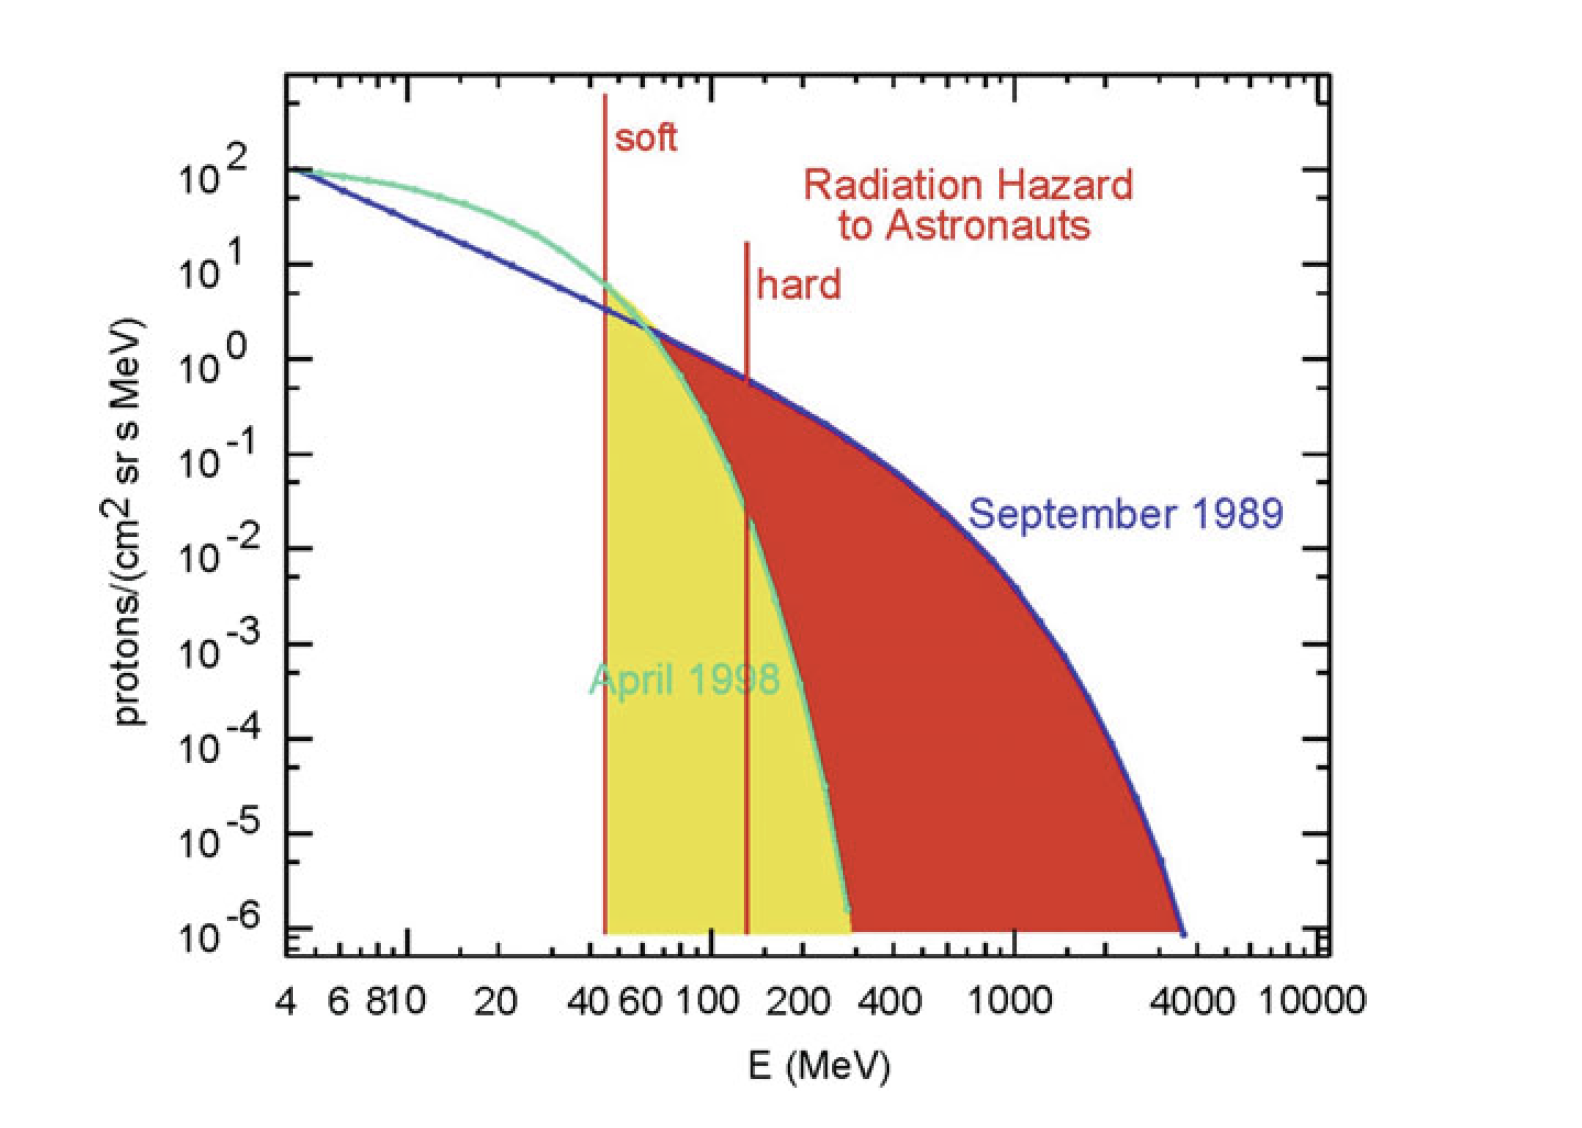
\includegraphics[width = 0.75\textwidth, height = 0.3\textheight]{images/SEP-radiation_hazard.png}
	\caption[The proton spectra in two \ac{SEP} events indicating the possible radiation energy]{The proton spectra of two famous \ac{SEP} events. The colored regions indicate the energy region with protons harmful to instruments and the human body. Both "hard" and "soft" spectra pose threats the human activities. (Figure reproduced from \citep{Reames2021LNP})}
	\label{Fig:SEP-radiation_hazard}
\end{figure}





% \section{Motivition}

% The inspiration of this thesis is from the following three aspects:
% \begin{itemize}
% 	\item New solar cycle: The recently solar minimum have ended in 2020 before the starting of th new \ac{SC} 25. Many observations haved already implied the unusual characteristics of this solar cycle. It is all known that the recent solar minimum have the most quite solar. The \ac{GCR} flux reached historically high levels in the space age \citep{Fu2021ApJS, Xu2022FrASS}, but ACR intensities did not reach such high, record-setting levels \citet{Strauss2023ApJ}. Moreover, the solar activities raised up rapidly and it could be the strongest \ac{SC} since records begin \citet{Nagovitsyn2023SoPh}. The peak of the solar cycle might arrive 1 year earlier than the prediction \citet{McIntosh2020SoPh}. On the other hand, after the solar minimum, the increasing solar eruptions and \ac{SEP} events provide researchers more oppurtunities to study the solar activities and their impact on the Earth and planet.
% 	\item New mission and new measurements: Over the last few years, several thrilled missions has been successfully launched after extensive preparation, such as \ac{PSP}, \ac{SolO}, \ac{Bepi}, lunar mission like Chang'E series mission, ESA's Jupiter Icy Moons Explorer - Juice, and Chinese missions like CHASE and ASO-S. In this thesis, we focused particularly on the new measurement from \ac{SolO} and \ac{LND}. The former provide the fantastic oppurtunities to study the solar activities in such a close distanc and the latter is the first human mission on the surface of Moon monitoring the radiation environment. The availability of those new observations could enhance our studies of the helioshphere.
% 	\item Multipoint observations in the heliosphere: With the increasing number of mission deployed in the space, multipoint observations is becoming more and more important and prevalent, enabling comprehensive moitoring of the solar activities at wide spread regions and at different radial distance. 
	
% \end{itemize}

% Therefore, following the idea of utilizing the new measurements from \ac{SolO} and \ac{LND}, in this thesis, we presents the first  observations of \ac{SEP} from \ac{LND} in Sec.~\ref{chp:LND_SEP}, \ac{GCR} and secondary proton measured on the lunar surface in Sec.~\ref{chp:LND_GCR_albedo}, quite time spectra (\ac{GCR}) measured in the inner heliosphere(Sec.~\ref{chp:SOLO_Quite_time})and the change of the \ac{ACR} helium radial gradient in the new solar cycles (Sec.\ref{chp:ACR_Helium}).
% The introduction of the instrument \ac{LND} and \ac{SolO}/\ac{HET} is given in Sec.~.\ref{chp:instruments}. The summary and outlook conclude this thesis. In particular, more detailed information of the \ac{LND} are provided in the Appendix ~\ref{chp:LNDinstrument}

% % The exploration of space has witnessed a surge in intensity, with an increasing number of countries aspiring to venture into this domain. Noteworthy examples include NASA's initiation of the Artemis mission, which aims to return to the Moon by 2024. Similarly, China has unveiled its plans to establish a lunar base on the lunar surface by the 2030s, while the European Space Agency (ESA) has also embarked on a lunar lander mission. Most recently, a Japanese lunar lander mission was launched; however, it regrettably encountered failure.

% % Under these circumstances, the study of solar energetic particles (SEPs) assumes greater significance. SEPs pose a significant radiation hazard for future human exploration on the lunar surface. The most hazardous SEP events have the potential to induce radiation increases of substantial magnitude.

% % SEP events directed towards Earth can become an issue of space weather and
% % very energetic events can cause a so-called Ground Level Enhancement (GLE).
% % This means that the radiation level on the ground increases which can be seen in
% % neutron monitor measurements.